\documentclass[technical_document.tex]{subfiles}
\begin{document}

\section{Design constraints}

To design the head, some tradeoffs between the visual appearance and the mechanical part had to be made. The head was designed in such a way that it is not only a cover, but also the ‘frame’ everything is connected to. One of the requirements for the head is expressing emotions. %TODO ref?
This is done by adding eyebrows, capable of moving . These eyebrows had to twist and to go up and down.  To stimulate the interaction between Eva and the people around her, her head is programmed to always look at the closest person in the room. For this functionality the head has to be able to pan and tilt.  %TODO sound / leds?

\section{Mechanical design}

\subsection{Eyebrows}
For the motion of the eyebrows, small hobby servos were used. On these servos a little block is mounted. These blocks are equipped with threaded holes. The eyebrows are mounted on a small aluminum shafts equipped with screw-thread, connected to the threaded holes on the servo. This allows the eyebrows to be removed by simply unscrewing them. The two mini servos are attached to a thin aluminum plate which is capable of providing the up-and-down movement. It is a bent plate made of 1mm thick aluminum. On the other side, this plate is attached to the main servo and bearings. Rotating the eyebrows turned out to work really well, but the up and down movement was problematic. Every time the Arduino\footnote{see http://arduino.cc} was initialized, the servo went from 0 degrees to 180 degrees which caused the servo to come loose of the head itself. This happened several times. Another problem was positioning inaccuracy. The servo never reached its target position. To fix this, the servo was disassembled and controlled using our own Arduino-based PID controller. This improved positioning accuracy, but soon started to give problems as well. Because of time constrains the eyebrows were decided to stay fixed at one position instead of being able to move up and down. In the future this feature could be re-implemented quite easily, as only the servo needs to be replaced with one of better quality.

\begin{figure}[ht!]
	\centering
	\mbox{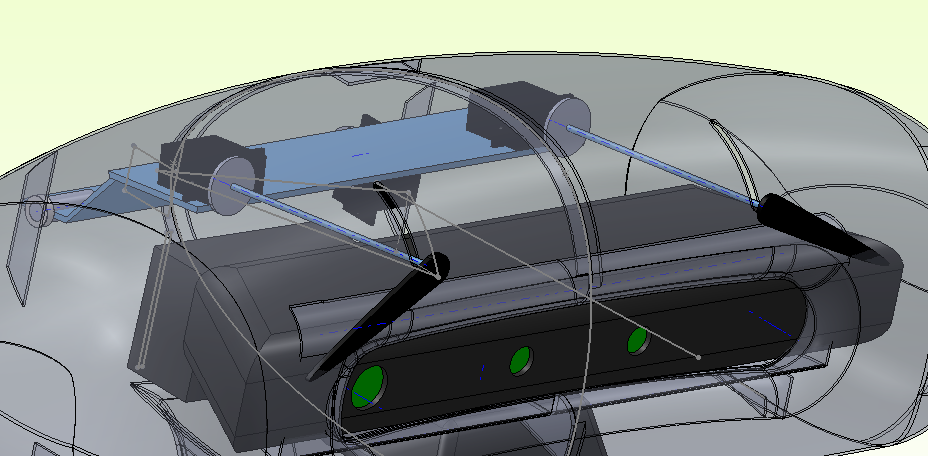
\includegraphics[scale=0.4]{Images/eyebrows_front.png}}
	\caption{Front view of the eyebrows}
	\label{fig:eyebrows_front}
\end{figure}

\begin{figure}[ht!]
	\centering
	\mbox{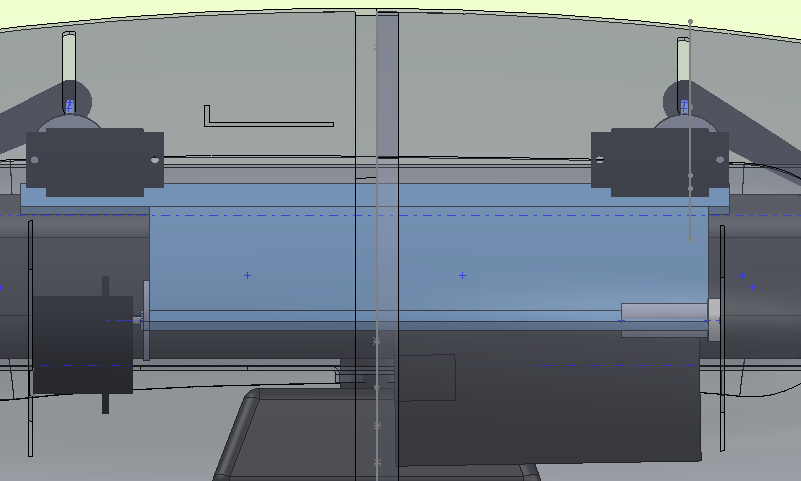
\includegraphics[scale=0.4]{Images/eyebrows_back.png}}
	\caption{Back view of the eyebrows}
	\label{fig:eyebrows_back}
\end{figure}

As shown in fig. \ref{fig:eyebrow_rotate} the torque which is needed for only rotating an eyebrow is $4.905*10^-5Nm$. This is not the only load on the servo. The eyebrow is mounted on a stick of $100mm$, which causes a bit of friction between the stick and the 3D-printed head. One of the cheapest hobby servos available already has a torque of about $0.10Nm$, over 2000 times more than the required rotational torque. Even including friction this was estimated to be enough. Some testing with the actual servos confirmed they were suitable. 

\begin{figure}[ht!]
	\centering
	\mbox{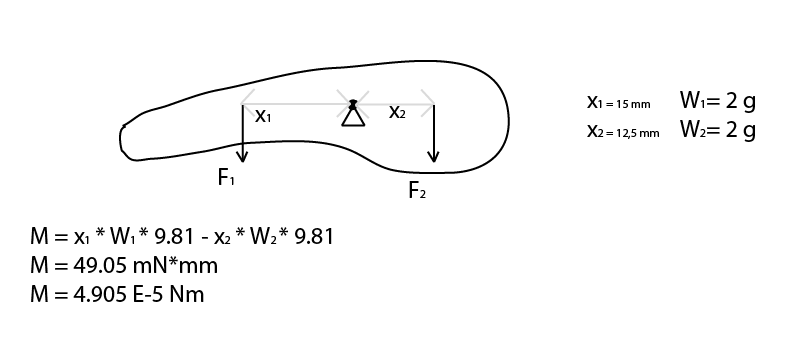
\includegraphics[scale=0.4]{Images/eyebrow_rotate.png}}
	\caption{Calculating the eyebrow rotation}
	\label{fig:eyebrow_rotate}
\end{figure}

As shown in fig. \ref{fig:eyebrow_upDown} the torque which is needed to move the eyebrows up and down is 0.051 Nm. Therefore a slightly stronger servo motor was chosen. The servo has a specified torque of 0.15 Nm, this proved to be strong enough for lifting the eyebrows.

\begin{figure}[ht!]
	\centering
	\mbox{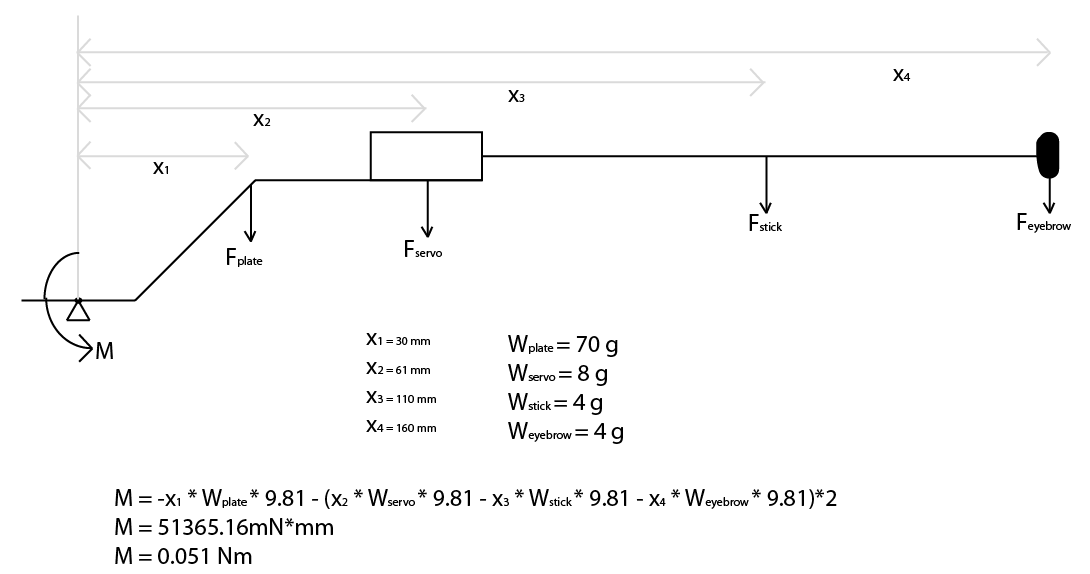
\includegraphics[scale=0.4]{Images/eyebrow_upDown.png}}
	\caption{Calculations of moving the eyebrows up and down}
	\label{fig:eyebrow_upDown}
\end{figure}


\subsection{Pan / tilt mechanism}

As mentioned in the paper %TODO reference to chapter / section?
hobby servo\textquotesingle{}s did not work to pan and tilt the head so we used two RX-28 dynamixels \footnote{see $http://www.crustcrawler.com/motors/RX28/docs/RX28_Manual.pdf$} %TODO is referencing via a footnote OK?
. These are much stronger than normal hobby servo\textquotesingle{}s and could turn more than 180 degrees if required. The dynamixels used have a holding torque of 2.78 Nm. To be sure this design would work, a few simple calculations\footnote{see sections \ref{subsection:tiltHead} and \ref{subsection:panHead}} were done to confirm these dynamixels would be suitable.


\begin{figure}[ht!]
	\centering
	\mbox{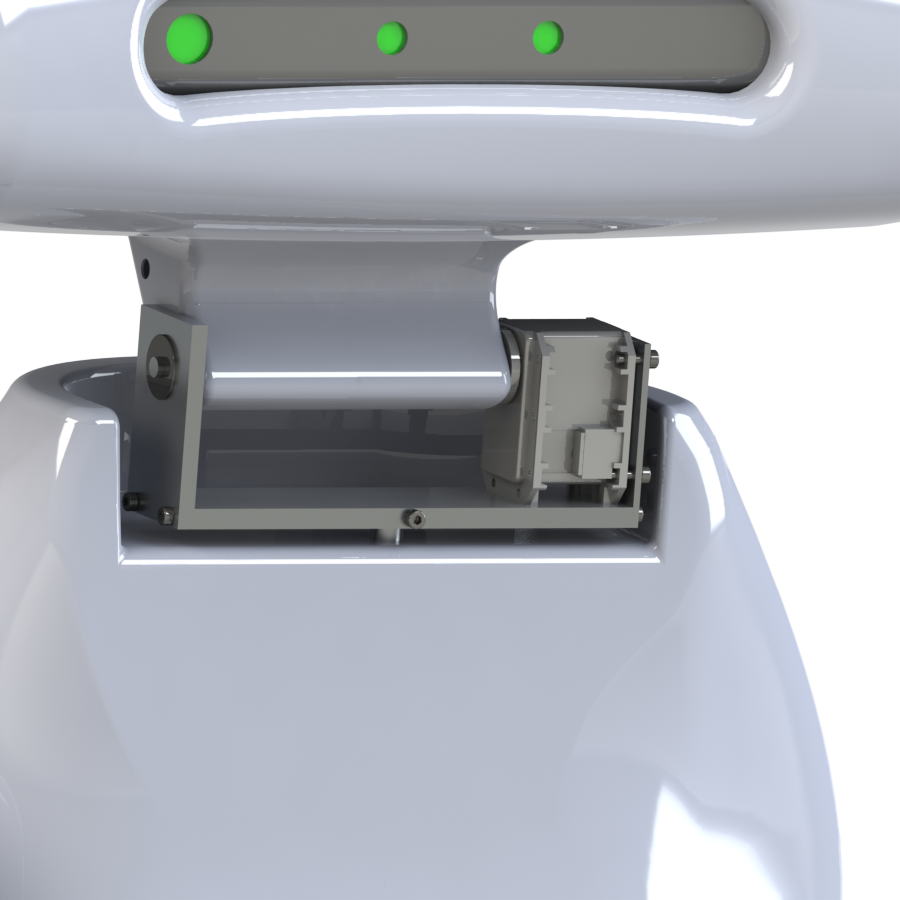
\includegraphics[scale=0.8]{Images/neck.png}}
	\caption{Final design of the pan/tilt mechanism}
	\label{fig:neck_final}
\end{figure}

To pan the head a solid aluminum plate was designed, which could be attached to an axle suspended by roller bearings. This vertical axle is attached to a dynamixel in the body, the other dynamixel is mounted on the plate. This dynamixel is placed directly next to the head and directly drives it.
This place was chosen because the dynamixel would not fit inside the head. On the opposite side of the upper dynamixel the head is supported by a bearing. This bearing connects to an axle running all the way from the left side to the right side of the head. This design worked really well, as expected. An extra advantage of using dynamixels is the position feedback, which turned out to be a very useful for improving the face tracking performance. %TODO reference to head tracking chapter
 

\subsubsection{Tilting the head}
\label{subsection:tiltHead}

\begin{figure}[ht!]
	\centering
	\mbox{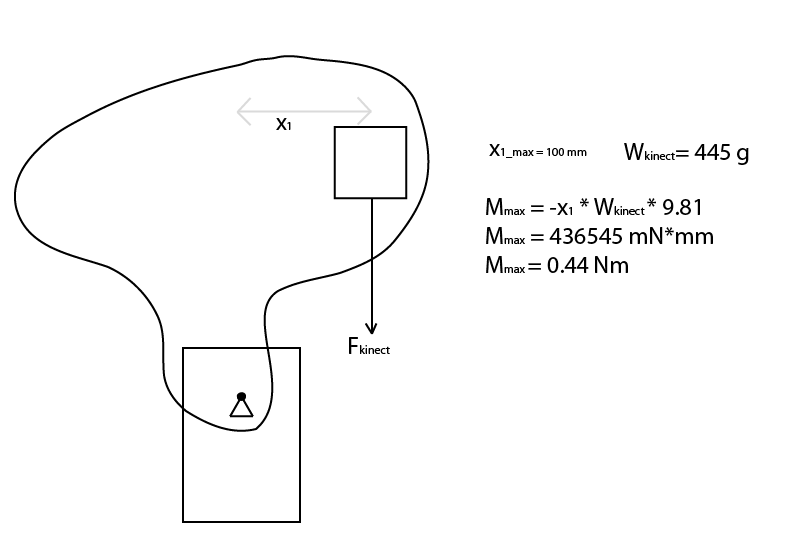
\includegraphics[scale=0.4]{Images/head_tilt.png}}
	\caption{Calculations of tilting the head}
	\label{fig:head_tilt}
\end{figure}

Fig. \ref{fig:head_tilt} shows the torque which is required for tilting the head. The Kinect is by far the heaviest
object in the head, which is also placed pretty far from the servo. Therefore the momentum on the neck is assumed to result mainly from the Kinect. As shown in the image, the required torque
for lifting the Kinect is $0.44Nm$. In the first design a normal servo with a maximum torque of $0.35Nm$ was used. The calculations clearly confirm this servo was not strong enough. The available dynamixel has a holding torque of $2.78Nm$, which should be more than enough for tilting the head.

\subsubsection{Panning the head}
\label{subsection:panHead}

To pan the head, the dynamixel has to overcome frictional forces and has to be strong enough to accelerate the head fast enough to be able to move the head smoothly. The frictional forces are unknown, but assumed to be very low, as the design will incorporate suitable bearings. Knowing
the maximum dynamixel torque and approximating the geometry of the head, an approximation for the angular acceleration can be made. The moment of inertia is approximated as that of a rectangular shape with the mass of around 1kg. The real moment of inertia is probably less, but would be very hard to calculate by hand. If the dynamixel is suitable for this calculation, it is definitely suitable for moving the real head.

\begin{figure}[ht!]
	\centering
	\mbox{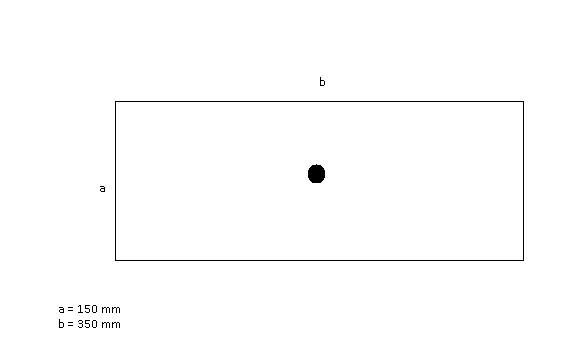
\includegraphics[scale=0.4]{Images/head_pan.png}}
	\caption{Calculations of panning the head}
	\label{fig:head_pan}
\end{figure}


As shown in Fig \ref{fig:head_pan} the potential angular acceleration is very high. The required acceleration would be a lot lower, because the code controlling the head limits acceleration at $2rad/s^2$. This suggests the panning dynamixel is more than strong enough. Testing confirmed this, it works really well.






\end{document}